% Primarily this section should be about scientific methods and theories you need to evaluate/compare/invent to solve your problems from 1.3.
% In some cases it may be ok to describe different technologies, but the purpose is to describe something and then draw a conclusion from that.
% Example, if you decide to discuss different databases, it may be for the purpose of selecting the best type for your implementation later on (based on for example data representation, scalability, speed, etc.).
% Optimally the problems in 1.3 are not solved by anyone else yet, in which case this section needs to describe how to solve them (new algorithms, mathematical approaches, etc.).
 
% This section can have a lot of subsections (3.1, 3.2, 3.3, etc).

% TODO: Explain Unwinding call stack

Virtually unwinding the call stack is done by recursively unwinding a stack of \emph{subroutine activations}.
It is called virtual unwinding because the state of the debugged target is not changed at any point during the unwinding.
Every subroutine in the call stack has a activation and a stack frame.
And because the activation often has the value of the stack pointer, the related stack frame is also known.
Thus successfully unwinding all the \emph{subroutine activations} will result in complete understanding of the state of the call stack.


The debug information needed to unwind activations are stored in the \gls{DWARF} section \emph{.debug\_frame}.
That section is made up of two data structures, one is called \gls{fde}.
A \gls{fde} contains a table used for unwinding registers and the \gls{cfa} of a activation.
The other data structure is called \gls{cie}, it contain information that is shared among many \glspl{fde}.
The relevant \gls{cie} and \gls{fde} to a activation can be found using the code location where it is stopped.


Unwinding the stack of activation is done by first evaluating the values of the top activation, read section \ref{sec:subact} to learn how that is done.
It starts with the top activation because there is to little information known of the other activations.
Next step is to find the \gls{cie} and \gls{fde} that contain debug info on the next activation.
When those are known the values of the next activation can be evaluated as describe in section \ref{sec:subact}.
This is then repeated for the rest of activation.


% ###############################################
\subsubsubsection{Subroutine Activation} \label{sec:subact}
A \emph{subroutine activation} contain information on a subroutine call/activation.
Each \emph{subroutine activation} contain a code location within the subroutine, it is the location where the subroutine stopped.
The reason for stopping could be that a breakpoint was hit, it was interrupted by a event or it could be location were it made a call to the next subroutine.


The address of the stopped code location is easily found using the stack pointer of the above activation in the activation stack.
Because the return address of the above activation is almost always stored on the stack.
This works for all activations except for the top activation, were stopped code location it is the current \gls{pc} value.


A activation also describe the state of some of the registers where it stopped.
Those are the registers that are preserved thanks to the prologue and epilogue code of the subroutine.
The rest of the registers are unknown because they have been written over, which makes them impossible to recover.


The activations is identified by there \gls{cfa} value. 
The \gls{cfa} is the value of the stack pointer in the previous stack frame.
One thing to note is that the \gls{cfa} is not the same value as the stack pointer when entering the current \emph{call frame}(see \cite{dwarf} page 126).


Both the values of the \gls{cfa} and the preserved register can be restored using tables located in the \gls{DWARF} section \emph{.debug\_frame}.
Checkout section \ref{sec:evalcfa} to learn how that is done.



% ###############################################
\subsubsubsection{Unwinding \gls{cfa} And Registers} \label{sec:evalcfa}
The tables in the \glspl{fde} contains virtual unwinding rules for a subroutine.
These virtual unwinding rules are used to restore the values of registers and the \gls{cfa}.


The first column in the tables contains code addresses, the addresses are used to identify the code location that all the virtual unwinding rules on that row applies for.
Next column is special because it contains the virtual unwinding rules for \gls{cfa}.
The rest of the columns contain the virtual unwinding rules for registers $0$ to $n$, where $n$ is the last registry.
Check out figure \ref{fig:stacktracetable} for a visual of how the tables are structured.


\begin{figure}[h]
	\centering
	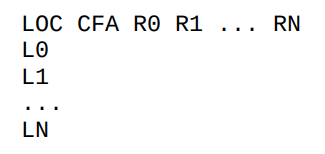
\includegraphics[width=0.5\textwidth]{stacktrace-table.png}
	\caption{This is how the table for reconstructing the \gls{cfa} and registers looks like. \emph{LOC} means that it is the column containing the code locations for $0$ to $N$. The column with \gls{cfa} has the virtual unwinding rules for \gls{cfa}. The rest of the column \emph{R0} to \emph{RN} holds all the virtual unwinding rules for the register $0$ to $N$.}
	\label{fig:stacktracetable}
\end{figure}


There are a number of different virtual unwinding rules, the ones for the registers are called register rules.
Some of them are very easy to use such as the register rule \emph{undefined}, this rules means that it is impossible to unwind that register.
Other ones require some calculations such as the register rule \emph{offset(N)}, where the \emph{N} is a signed offset.
This rule means that the register value is stored at the \gls{cfa} address plus the offset $N$.
All of the rules can be read about in the \gls{DWARF} specification \cite{dwarf} on page 128.


Unwind a register is done by first finding the correct row.
That is done by finding the closes address that is less then the search one.
Next step is to evaluate the new value using the register rule on the row.
Then go to the next row in the table and do the same thing but with the new value.
Repeat until there are now more rows.
That is how to use the table to unwind a register.

